\documentclass[12pt,a4paper]{article}

% ─── Page Layout ───────────────────────────────────────────────────────────────
\usepackage[a4paper, margin=0.8in, headheight=14pt]{geometry}

% ─── Fonts (XeLaTeX) ───────────────────────────────────────────────────────────
\usepackage{fontspec}
\usepackage{unicode-math}
\setmainfont{TeX Gyre Pagella}
\setmonofont[Scale=0.88]{TeX Gyre Cursor}
\setmathfont{Latin Modern Math}

% ─── Packages ──────────────────────────────────────────────────────────────────
\usepackage{xcolor}
\usepackage{colortbl}
\usepackage{titlesec}
\usepackage{enumitem}
\usepackage{tabularx}
\usepackage{booktabs}
\usepackage{array}
\usepackage{amsmath}
\usepackage{tikz}
\usetikzlibrary{shapes.geometric, arrows.meta, positioning, calc, fit, decorations.pathreplacing}
\usepackage{tcolorbox}
\tcbuselibrary{skins, breakable}
\usepackage{hyperref}
\usepackage{fancyhdr}
\usepackage{graphicx}
\usepackage{microtype}
\hyphenpenalty=10000
\exhyphenpenalty=10000
\sloppy
\usepackage{caption}
\usepackage{setspace}
\usepackage{multirow}
\usepackage{tocloft}

% ─── Q&A helper ────────────────────────────────────────────────────────────────
\newcommand{\Q}[1]{\textbf{#1}\par\noindent\ignorespaces}

% ─── Colour Palette ────────────────────────────────────────────────────────────
\definecolor{myred}{RGB}{196,30,58}
\definecolor{mydark}{RGB}{30,30,50}
\definecolor{mygreen}{RGB}{14,120,80}
\definecolor{myteal}{RGB}{0,130,140}
\definecolor{myamber}{RGB}{180,100,0}
\definecolor{mypurple}{RGB}{100,30,160}
\definecolor{mygray}{RGB}{246,247,249}
\definecolor{mgframe}{RGB}{180,185,200}
\definecolor{watermark}{RGB}{145,150,170}
\definecolor{hdrred}{RGB}{250,232,235}
\definecolor{hdrgreen}{RGB}{220,244,233}
\definecolor{hdrteal}{RGB}{220,242,244}
\definecolor{hdramber}{RGB}{253,242,215}
\definecolor{hdrpurple}{RGB}{238,228,255}
\definecolor{hdrgray}{RGB}{238,240,245}
\definecolor{rowalt}{RGB}{250,251,253}

% ─── Section Formatting ────────────────────────────────────────────────────────
\titleformat{\section}
  {\large\bfseries\color{myred}}{\thesection.}{0.5em}{}
  [\vspace{1pt}{\color{myred}\rule{\linewidth}{0.8pt}}]
\titleformat{\subsection}
  {\normalsize\bfseries\color{myteal}}{\thesubsection}{0.5em}{}
\titlespacing*{\section}{0pt}{18pt}{7pt}
\titlespacing*{\subsection}{0pt}{11pt}{4pt}

% ─── Paragraph ─────────────────────────────────────────────────────────────────
\setlength{\parindent}{0pt}
\setlength{\parskip}{4pt}

% ─── TOC Styling ───────────────────────────────────────────────────────────────
\renewcommand{\cfttoctitlefont}{\large\bfseries\color{myred}}
\renewcommand{\cftaftertoctitle}{\par\noindent{\color{myred}\rule{\linewidth}{0.8pt}}}
\setlength{\cftbeforetoctitleskip}{0pt}
\setlength{\cftaftertoctitleskip}{6pt}
\renewcommand{\cftsecfont}{\normalsize\bfseries\color{mydark}}
\renewcommand{\cftsecpagefont}{\normalsize\bfseries\color{mydark}}
\renewcommand{\cftsecleader}{\cftdotfill{\cftdotsep}}
\setlength{\cftbeforesecskip}{7pt}
\renewcommand{\cftsubsecfont}{\small\color{mydark}}
\renewcommand{\cftsubsecpagefont}{\small\color{mydark}}
\setlength{\cftbeforesubsecskip}{3pt}
\setlength{\cftsubsecindent}{1.4em}

% ─── Table helpers ─────────────────────────────────────────────────────────────
\renewcommand{\arraystretch}{1.45}
\setlength{\tabcolsep}{6pt}
\arrayrulecolor{mydark}
\newcolumntype{B}[1]{>{\small\bfseries\raggedright\arraybackslash}m{#1}}
\newcolumntype{Y}{>{\small\raggedright\arraybackslash}X}
\renewcommand{\tabularxcolumn}[1]{m{#1}}

% ─── Header / Footer ───────────────────────────────────────────────────────────
\pagestyle{fancy}
\fancyhf{}
\fancyhead[L]{\small\color{myred}\textbf{PE-EC701A}\;\color{mydark}--- Microwave Theory and Technique}
\fancyhead[R]{\small\color{myteal}\textbf{Module 9 Notes}}
\fancyfoot[C]{\small\color{mydark}\thepage}
\fancyfoot[R]{\small\color{watermark}\textit{\copyright\ Biraj}}
\renewcommand{\headrulewidth}{0.5pt}
\renewcommand{\footrulewidth}{0.3pt}

% ─── Hyperref ──────────────────────────────────────────────────────────────────
\hypersetup{
  colorlinks=true, linkcolor=myteal, urlcolor=myteal,
  pdfauthor={Biraj Sarkar},
  pdftitle={PE-EC701A --- Module 9 Notes}
}

% ─── tcolorbox styles ──────────────────────────────────────────────────────────
\tcbset{
  tikzbox/.style={
    colback=mygray, colframe=mgframe, boxrule=0.6pt, arc=4pt,
    left=8pt, right=8pt, top=6pt, bottom=6pt,
    colbacktitle=mgframe, coltitle=mydark,
    fonttitle=\small\bfseries
  },
  defbox/.style={
    colback=hdrgreen, colframe=mygreen, boxrule=0.8pt, arc=4pt,
    left=9pt, right=9pt, top=6pt, bottom=6pt,
    colbacktitle=mygreen, coltitle=white,
    fonttitle=\small\bfseries
  },
  formulabox/.style={
    colback=hdrteal, colframe=myteal, boxrule=0.8pt, arc=4pt,
    left=9pt, right=9pt, top=7pt, bottom=7pt,
    colbacktitle=myteal, coltitle=white,
    fonttitle=\small\bfseries
  },
  examplebox/.style={
    colback=hdramber, colframe=myamber, boxrule=0.8pt, arc=4pt,
    left=9pt, right=9pt, top=6pt, bottom=6pt,
    colbacktitle=myamber, coltitle=white,
    fonttitle=\small\bfseries
  },
  masonbox/.style={
    colback=hdrpurple, colframe=mypurple, boxrule=0.8pt, arc=4pt,
    left=9pt, right=9pt, top=6pt, bottom=6pt,
    colbacktitle=mypurple, coltitle=white,
    fonttitle=\small\bfseries
  },
  exambox/.style={
    colback=hdrpurple, colframe=mypurple, boxrule=1pt, arc=5pt,
    left=10pt, right=10pt, top=8pt, bottom=8pt,
    colbacktitle=mypurple, coltitle=white,
    fonttitle=\bfseries,
    breakable, title after break={\textbf{Frequently Asked / Viva Questions (contd.)}}}
}
% Make all boxes breakable across pages
\tcbset{breakable}

% ─── TikZ styles ───────────────────────────────────────────────────────────────
\tikzset{
  block/.style={rectangle, draw=myteal, fill=hdrteal,
    text width=2.4cm, align=center, minimum height=0.95cm,
    font=\small, rounded corners=3pt, line width=0.7pt},
  redblock/.style={rectangle, draw=myred, fill=hdrred,
    text width=2.4cm, align=center, minimum height=0.95cm,
    font=\small, rounded corners=3pt, line width=0.7pt},
  netnode/.style={rectangle, draw=myteal, fill=hdrteal,
    text width=1.5cm, align=center, minimum height=0.8cm,
    font=\small, rounded corners=3pt, line width=0.7pt},
  sumjunc/.style={circle, draw=myamber, fill=hdramber,
    minimum size=0.62cm, font=\small, line width=0.8pt},
  snode/.style={circle, draw=mypurple, fill=hdrpurple,
    minimum size=0.55cm, font=\footnotesize, line width=0.7pt},
  arrow/.style={-Stealth, thick, color=mydark},
  redarrow/.style={-Stealth, thick, color=myred},
  line/.style={thick, color=mydark}
}

% ═══════════════════════════════════════════════════════════════════════════════
\begin{document}
% ═══════════════════════════════════════════════════════════════════════════════

\begin{center}
  {\LARGE\bfseries\color{myred} PE-EC701A --- Microwave Theory and Technique}\\[5pt]
  {\normalsize\color{mydark} Semester VII \quad$\bullet$\quad 3L:0T:0P \quad$\bullet$\quad 3 Credits}\\[3pt]
  {\normalsize\color{myteal}\textbf{Module 9 Exam Notes: Microwave Systems \& Modern Trends}}\\[3pt]
  {\small\color{mydark} CGEC \;$|$\; B.Tech ECE (2023--27) \;$|$\; \textit{Biraj Sarkar}}
\end{center}
\vspace{2pt}
\noindent{\color{myred}\rule{\linewidth}{1.5pt}}
\vspace{2pt}

\hypersetup{linkcolor=mydark}
\tableofcontents
\hypersetup{linkcolor=myteal}
\newpage

% ===============================================================================
\section{Radar Systems}
% ===============================================================================

RADAR (RAdio Detection And Ranging) is an active electromagnetic system that transmits microwave pulses and processes reflections to determine target range, velocity, and angle.

\begin{tcolorbox}[tikzbox, title={Pulsed Radar Block Diagram}]
\centering
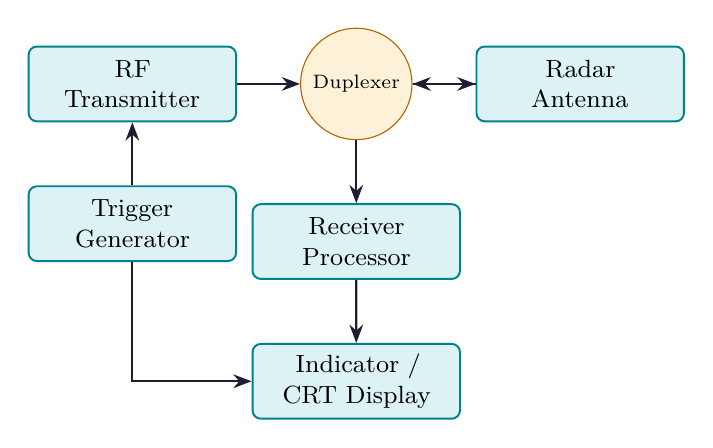
\begin{tikzpicture}[scale=0.9, every node/.style={font=\scriptsize}]
  \node[block] (tx) {RF\\Transmitter};
  \node[block, below=0.8cm of tx] (trg) {Trigger\\Generator};
  \node[circle, draw=myamber, fill=hdramber, right=0.8cm of tx, minimum size=0.8cm] (dup) {Duplexer};
  \node[block, right=0.8cm of dup] (ant) {Radar\\Antenna};
  \node[block, below=0.8cm of dup] (rx) {Receiver\\Processor};
  \node[block, below=0.8cm of rx] (dsp) {Indicator /\\CRT Display};
  
  \draw[arrow] (tx) -- (dup);
  \draw[arrow] (dup) -- (ant);
  \draw[arrow] (ant) -- (dup); % Return path
  \draw[arrow] (dup) -- (rx);
  
  \draw[arrow] (trg) -- (tx);
  \draw[arrow] (trg) |- (dsp);
  \draw[arrow] (rx) -- (dsp);
\end{tikzpicture}
\end{tcolorbox}

\begin{tcolorbox}[formulabox, title={\textbf{Radar Range Equation}}]
The maximum radar detection range $R_{\text{max}}$ is given by:
\begin{equation}
  R_{\text{max}} = \left[ \frac{P_t G^2 \lambda^2 \sigma}{(4\pi)^3 P_{\text{min}}} \right]^{\!1/4} \quad (\text{m})
\end{equation}
Where:
\begin{itemize}[leftmargin=1.5em, itemsep=1pt, topsep=2pt]
  \item[] $P_t$ = peak transmitter power (W)
  \item[] $G$ = antenna gain
  \item[] $\lambda$ = RF operating wavelength (m)
  \item[] $\sigma$ = Radar Cross Section (RCS) of target ($\text{m}^2$)
  \item[] $P_{\text{min}}$ = minimum detectable receiver signal (W)
\end{itemize}
\end{tcolorbox}

\textbf{Radar Variations:}
\begin{enumerate}[leftmargin=*, itemsep=3pt]
  \item \textbf{CW (Continuous Wave) Radar:} Transmits continuously, measures velocity using \textbf{Doppler shift} ($f_d = 2v/\lambda$).
  \item \textbf{FMCW (Frequency Modulated CW) Radar:} Sweeps transmitter frequency, allowing both range and velocity to be measured.
  \item \textbf{MTI (Moving Target Indicator) Radar:} Suppresses static clutter (ground, buildings) using delay-line cancelers.
\end{enumerate}

% ===============================================================================
\section{Terrestrial and Satellite Communications}
% ===============================================================================

\begin{tcolorbox}[tikzbox, title={Satellite Uplink/Downlink Path Schematic}]
\centering
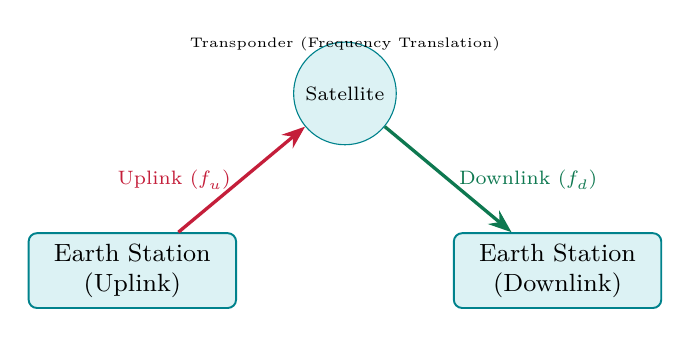
\begin{tikzpicture}[scale=0.9, every node/.style={font=\scriptsize}]
  \node[draw=myteal, fill=hdrteal, circle, minimum size=1.0cm] (sat) at (3,2.5) {Satellite};
  \node[block] (es1) at (0,0) {Earth Station\\(Uplink)};
  \node[block] (es2) at (6,0) {Earth Station\\(Downlink)};
  
  \draw[arrow, color=myred, line width=1.2pt] (es1) -- (sat) node[midway, left] {Uplink ($f_u$)};
  \draw[arrow, color=mygreen, line width=1.2pt] (sat) -- (es2) node[midway, right] {Downlink ($f_d$)};
  
  \node[font=\tiny] at (3, 3.2) {Transponder (Frequency Translation)};
\end{tikzpicture}
\end{tcolorbox}

\textbf{Link Budget ($C/N$):} Carrier-to-Noise ratio at the receiver terminal:
  \begin{equation}
    \left(\frac{C}{N}\right)_{\text{dB}} = \text{EIRP}_{\text{dBW}} + \left(\frac{G}{T}\right)_{\text{dB/K}} - \text{FSL}_{\text{dB}} - k_{\text{dBW}} - B_{\text{dB-Hz}}
  \end{equation}
  where $\text{EIRP}$ is Equivalent Isotropic Radiated Power, $G/T$ is receiver figure of merit, $\text{FSL} = (4\pi d/\lambda)^2$ is Free Space Path Loss, and $k$ is Boltzmann's constant.

% ===============================================================================
\section{Radio Aids to Navigation}
% ===============================================================================

\begin{itemize}[leftmargin=*, itemsep=3pt]
  \item \textbf{GPS (Global Positioning System):} Employs 24+ satellites. Receivers measure transit times of signals from 4+ satellites, using \textbf{triangulation} to resolve latitude, longitude, altitude, and clock bias.
  \item \textbf{ILS (Instrument Landing System):} Provides guidance for aircraft landing: \textbf{Localizer} (lateral guidance, 108--112 MHz) and \textbf{Glide Slope} (vertical guidance, 329--335 MHz).
  \item \textbf{LORAN (Long Range Navigation):} Hyperbolic radio navigation system using time-difference arrivals of pulses from ground stations.
  \item \textbf{RFID (Radio Frequency Identification):} Uses electromagnetic coupling in microwave/RF bands for asset tracking.
\end{itemize}

% ===============================================================================
\section{Modern Trends: Biological Effects, MMICs, and RFMEMS}
% ===============================================================================

\begin{itemize}[leftmargin=*, itemsep=3pt]
  \item \textbf{Biological Effects \& SAR:} Microwaves cause dielectric heating of tissues. The \textbf{SAR (Specific Absorption Rate)} measures RF energy absorption by body tissues:
    \begin{equation}
      \text{SAR} = \frac{\sigma |E|^2}{\rho} \quad (\text{W/kg})
    \end{equation}
    where $\sigma$ is tissue conductivity, $E$ is electric field, and $\rho$ is mass density. Regulatory limits are typically $1.6\text{ W/kg}$ over $1\text{ g}$ of tissue.
  \item \textbf{MMICs:} Monolithic Microwave Integrated Circuits integrate passive components, transmission lines, and active transistors onto a single semiconductor substrate (GaAs, GaN, SiGe).
  \item \textbf{RFMEMS:} Micro-Electro-Mechanical Systems designed for RF/microwave signals. They offer high isolation, low insertion loss, and low power consumption.
  \item \textbf{Microwave Imaging:} A non-invasive imaging technique that maps the spatial distribution of dielectric properties (permittivity and conductivity) inside a body.
  \begin{itemize}[leftmargin=*, itemsep=2.5pt, topsep=0pt]
    \item \textbf{Active Imaging (Radar-based):} Transmits low-power microwave pulses and records the backscattered signals to reconstruct a 3D profile of dielectric contrasts.
    \item \textbf{Passive Imaging (Radiometry):} Detects natural thermal microwave radiation emitted by the body using ultra-sensitive radiometers.
    \item \textbf{Applications:} Non-destructive testing, airport security scanners (millimeter-wave body scanning), and medical diagnostics (such as breast cancer screening, which leverages the 5:1 permittivity contrast between high-water-content tumors and normal fat tissue).
  \end{itemize}
\end{itemize}

\begin{tcolorbox}[tikzbox, title={RFMEMS Capacitive Switch Model}]
\centering
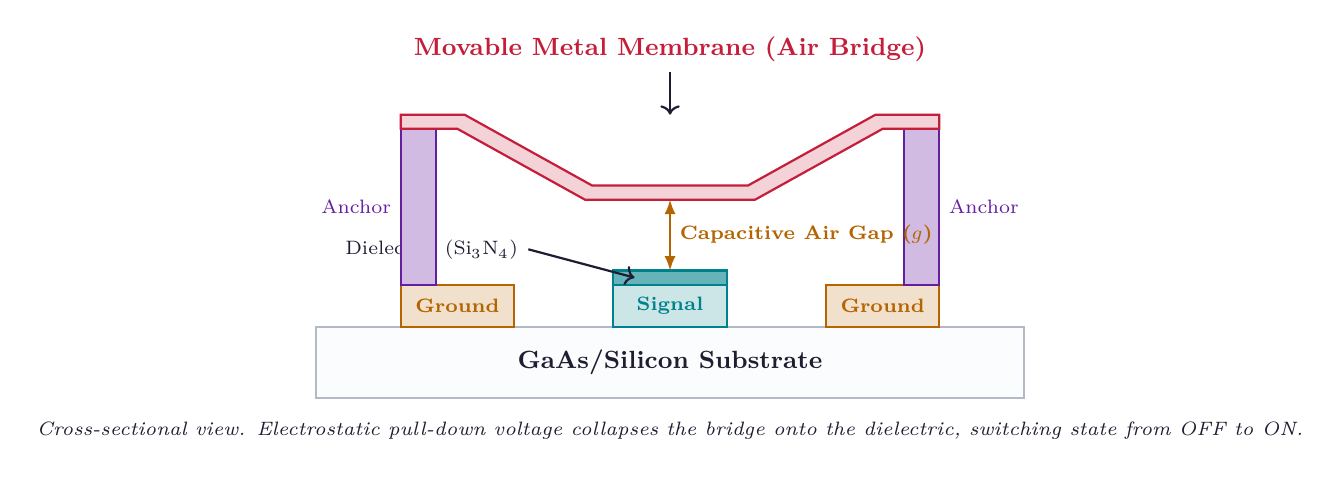
\begin{tikzpicture}[scale=0.9, every node/.style={font=\small}]
  % Substrate
  \draw[thick, fill=mygray!40, draw=mgframe] (0,0) rectangle (10,1.0);
  \node[font=\small\bfseries\color{mydark}] at (5,0.5) {GaAs/Silicon Substrate};

  % CPW Ground Electrodes
  \draw[thick, fill=myamber!20, draw=myamber] (1.2,1.0) rectangle (2.8,1.6);
  \node[font=\scriptsize\bfseries\color{myamber}] at (2.0,1.3) {Ground};
  
  \draw[thick, fill=myamber!20, draw=myamber] (7.2,1.0) rectangle (8.8,1.6);
  \node[font=\scriptsize\bfseries\color{myamber}] at (8.0,1.3) {Ground};

  % CPW Signal Electrode
  \draw[thick, fill=myteal!20, draw=myteal] (4.2,1.0) rectangle (5.8,1.6);
  \node[font=\scriptsize\bfseries\color{myteal}] at (5.0,1.3) {Signal};

  % Dielectric Layer on Signal (CRITICAL for capacitive switch)
  \draw[thick, fill=myteal!60, draw=myteal] (4.2,1.6) rectangle (5.8,1.8);
  \draw[arrow, <-] (4.5, 1.7) -- (3.0, 2.1) node[left, font=\scriptsize] {Dielectric ($\text{Si}_3\text{N}_4$)};

  % Anchors (Left & Right)
  \draw[thick, fill=mypurple!30, draw=mypurple] (1.2,1.6) rectangle (1.7,3.8);
  \draw[thick, fill=mypurple!30, draw=mypurple] (8.3,1.6) rectangle (8.8,3.8);
  \node[left, font=\scriptsize\color{mypurple}] at (1.2,2.7) {Anchor};
  \node[right, font=\scriptsize\color{mypurple}] at (8.8,2.7) {Anchor};

  % Suspended Bridge (Air Bridge Membrane)
  \draw[thick, fill=myred!20, draw=myred] 
    (1.2,3.8) -- (2.0,3.8) -- (3.8,2.8) -- (6.2,2.8) -- (8.0,3.8) -- (8.8,3.8) --
    (8.8,4.0) -- (7.9,4.0) -- (6.1,3.0) -- (3.9,3.0) -- (2.1,4.0) -- (1.2,4.0) -- cycle;

  % Labels and arrows
  \draw[arrow, <-] (5.0, 4.0) -- (5.0, 4.6) node[above, color=myred, font=\small\bfseries] {Movable Metal Membrane (Air Bridge)};
  
  % Capacitive Coupling Air Gap
  \draw[latex-latex, thick, color=myamber] (5.0,1.8) -- (5.0,2.8);
  \node[right, font=\scriptsize\bfseries\color{myamber}] at (5.0, 2.3) {Capacitive Air Gap ($g$)};

  % Switch State description
  \node[below, font=\scriptsize\itshape\color{mydark}] at (5,-0.2) 
    {Cross-sectional view. Electrostatic pull-down voltage collapses the bridge onto the dielectric, switching state from OFF to ON.};
\end{tikzpicture}
\end{tcolorbox}

% ===============================================================================
% MANDATORY QUICK REVISION PAGE
% ===============================================================================
\newpage
\begin{center}
  {\large\bfseries\color{myred} Quick Revision --- Module IX}\\[3pt]
  {\small\color{mydark} Microwave Systems \& Modern Trends $|$ PE-EC701A}
\end{center}
\noindent{\color{myred}\rule{\linewidth}{1.2pt}}
\vspace{4pt}

\begin{tcolorbox}[formulabox, title={\textbf{Key Formulas at a Glance}}]
\renewcommand{\arraystretch}{1.3}
\begin{tabularx}{\linewidth}{B{4.5cm} X}
Radar Range Equation   & $R_{\text{max}} = \left[ \frac{P_t G^2 \lambda^2 \sigma}{(4\pi)^3 P_{\text{min}}} \right]^{1/4}$ \\[4pt]
Doppler Frequency Shift & $f_d = \frac{2 v}{\lambda} \cos \theta$ \\[4pt]
Free Space Path Loss    & $\text{FSPL} = \left(\frac{4\pi d}{\lambda}\right)^{\!2}$ \\[4pt]
Specific Absorption Rate& $\text{SAR} = \frac{\sigma |E|^2}{\rho}$ \\[4pt]
Shielding Effectiveness & $\text{SE}_{\text{dB}} \approx A_{\text{dB}} + R_{\text{dB}} + M_{\text{dB}}$
\end{tabularx}
\tcbset{colbacktitle=mygreen, coltitle=white}
\end{tcolorbox}

\begin{tcolorbox}[defbox, title={\textbf{One-Line Definitions}}]
\begin{itemize}[leftmargin=*, itemsep=2.5pt, topsep=0pt]
  \item \textbf{Duplexer:} A fast waveguide switch permitting a single antenna to be shared by radar transmitter and receiver.
  \item \textbf{Doppler Effect:} The change in frequency of a received wave due to relative motion between source and observer.
  \item \textbf{SAR:} Specific Absorption Rate, measuring the rate of electromagnetic energy absorption per unit mass of human tissue.
  \item \textbf{MMIC:} Monolithic Microwave Integrated Circuit, fabricated entirely on a single semiconductor wafer.
  \item \textbf{RFMEMS:} Micro-Electro-Mechanical Systems utilized for high-performance microwave switching and tuning.
  \item \textbf{Triangulation:} Geometric position mapping utilizing measured transit distances from multiple satellites.
  \item \textbf{Clutter:} Unwanted reflections from ground objects, weather, or buildings that interfere with target radar signals.
  \item \textbf{Microwave Imaging:} A non-invasive imaging method mapping dielectric property contrasts within a target.
\end{itemize}
\end{tcolorbox}

\begin{tcolorbox}[exambox, title={\textbf{Frequently Asked / Viva Questions}}]
\begin{enumerate}[topsep=0pt, label=\textbf{Q\arabic*.}, itemsep=5pt]
  \item \Q{Why is a duplexer critical in pulsed radar systems?}
    It isolates the sensitive receiver from the high-power transmitter during the pulse transmission, and routes the weak return echo to the receiver during the rest interval.
  \item \Q{How does Doppler shift change with target movement direction?}
    If the target moves toward the radar, the received frequency increases ($+f_d$). If it moves away, the received frequency decreases ($-f_d$).
  \item \Q{Explain the term "Specific Absorption Rate" (SAR).}
    It is the power absorbed per unit mass of human tissue under RF exposure, measured in W/kg, used to define safety standards for mobile devices.
  \item \Q{What are the advantages of MMICs over hybrid Microwave Integrated Circuits (HMICs)?}
    Small size, low weight, high reliability, ease of mass production, and elimination of wire bond parasitics.
  \item \Q{Describe the function of localizer and glide path transmitters in ILS.}
    The localizer provides horizontal guidance relative to the runway centerline. The glide path provides vertical descent guidance to the runway touchdown point.
  \item \Q{Why does Free Space Path Loss (FSPL) increase with frequency?}
    Because effective antenna aperture decreases as frequency increases ($A_e \propto 1/f^2$), reducing the power intercepted by a matched receiving antenna.
  \item \Q{What are blind speeds in MTI radar and how are they avoided?}
    Blind speeds are target velocities where the Doppler shift matches the radar pulse repetition frequency, making targets appear static. They are avoided by using staggered PRFs.
  \item \Q{What materials are primarily used to fabricate MMICs and why?}
    Gallium Arsenide (GaAs) and Gallium Nitride (GaN) due to high electron mobility, which is necessary for gigahertz operation.
  \item \Q{How does a capacitive RFMEMS switch operate?}
    An electrostatic voltage pulls a suspended metal bridge down onto a dielectric-covered CPW line, dramatically increasing coupling capacitance to short the RF signal.
  \item \Q{Explain how GPS resolves a 3D position using four satellites.}
    Three satellites locate the receiver at the intersection of three spheres. The fourth satellite resolves the clock synchronization error between the receiver and GPS time.
  \item \Q{State the thermal effects of microwaves on the human body.}
    Dielectric heating of water molecules in body tissues, which can lead to localized temperature increases and tissue damage (especially in the eyes and testes).
  \item \Q{What is shielding effectiveness (SE) and what are its main mechanisms?}
    It measures a barrier's ability to attenuate electromagnetic fields, governed by absorption loss, reflection loss, and multiple-reflection corrections.
  \item \Q{Differentiate between active and passive microwave imaging.}
    Active microwave imaging transmits low-power microwave pulses and measures backscattered signals to reconstruct a dielectric profile. Passive microwave imaging uses highly sensitive radiometers to detect the natural thermal electromagnetic radiation emitted by the body.
  \item \Q{Why is microwave imaging promising for breast cancer detection?}
    Because malignant tumors have a high water content and thus show a significant dielectric contrast (permittivity and conductivity are about 5 times higher) compared to normal healthy breast fat tissue. This allows clear imaging without ionizing X-ray radiation.
\end{enumerate}
\tcbset{colbacktitle=mgframe, coltitle=mydark}
\end{tcolorbox}

\begin{tcolorbox}[tikzbox, title={Comparison of MMICs and Hybrid MICs}]
\renewcommand{\arraystretch}{1.4}
\par\noindent
\begin{tabularx}{\linewidth}{|B{3.2cm}|Y|Y|}
\hline
\rowcolor{hdrgray}
\textbf{Parameter} & \textbf{Monolithic Microwave ICs (MMICs)} & \textbf{Hybrid Microwave ICs (HMICs)} \\
\hline
\textbf{Substrate} & Single semiconductor wafer (GaAs, GaN). & Alumina, quartz, or Teflon board. \\
\hline
\rowcolor{rowalt}
\textbf{Component Integration} & Transistors and matching lines are grown in-situ on the wafer. & Discrete chips are soldered or wire-bonded to substrate tracks. \\
\hline
\textbf{Reliability} & Extremely high (no wire bonds to fail). & Moderate (wire bonds are vulnerable). \\
\hline
\rowcolor{rowalt}
\textbf{Cost (Low Volume)} & Very High (complex mask tooling). & Moderate (easy prototyping). \\
\hline
\textbf{Cost (High Volume)} & Very Low (mass batch production). & High (requires manual/auto assembly). \\
\hline
\end{tabularx}
\end{tcolorbox}

\end{document}
